\cotefile{119}
\scanpage{144}
% archive foliation: 143
\margin{(\unsure{15|17} p)}

Notes de math.\par
\unsure{oubliées} par Jean\par
Malgoire

\scanpage{145}
% archive foliation: 144
\margin{\uline{\unsure{Mettre où}}}
\margin{\fbox{Mars 1986}\quad\fbox{\begin{tabular}{c}``Feuille-\\tages''\end{tabular}}}

\uline{Topos quotient} d'un espace \inserted{$E$ [ou topos ?]} par une
\unsure{relation} d'\unsure{équivce} locale \inserted{$R$}
(ex: feuilletages de variétés). On trouve comme
quotients les espaces de la forme $(X,G)$, $X$ espace, $G$ gr. \unsure{qq}
discret opérant sur $X$ (\unsure{en ordinaire},
$G$ est le groupe fondamental d'une ``feuille''\ldots)
[Cas où toutes les feuilles \inserted{$F_i$} sont \unsure{homéom.},
et \unsure{où on a} $E\longrightarrow F$ induisant des
\uline{iso} $F_i\unsure{-|\longrightarrow}F$\ldots]

\margin{\unsure{N. définition|N. question} de l'holonomie\ldots}

\scanpage{146}
% archive foliation: 145
\margin{(\unsure{2-fonctorique}) \illegible{5}}

\uline{Th} Soit $C$ la catégorie des \inserted{$(X\unsure{,}R),X$}
esp. top. \deleted{\illegible{1}} et $R$ rel. d'\unsure{équivce}
locale sur $X$ [localement] ouvert à fibres loc.
connexes \deleted{\illegible{2}} \deleted{\illegible{1}}
(flèches : appl. continues comp. aux rel.
d'équiv. locales\ldots), et $C'$ la catégorie des
\deleted{\unsure{flèches}} \deleted{\illegible{1}} systèmes $(X,Y,f)$,
où $X$ espace top. \deleted{\illegible{1}},
$Y$ mult. top., $f:\operatorname{Top}(X)\longrightarrow\unsure{\mathcal{Y}|Y}$
morphisme qui est \inserted{(loc\textsuperscript{t})} ouvert,
à fibres loc\textsuperscript{t} connexes \uline{et}
connexes (flèches de $C'$ : \ldots c'est une $2$-cat.
où les \uline{$\operatorname{Hom}$}$(\xi,\eta)$ sont des cat. \uline{discrètes}). On a
\diagram{\begin{tikzcd}
C \arrow[r,shift right=0.7ex,"\approx"'] & C' \arrow[l,shift right=0.7ex,"\approx"']
\end{tikzcd}}.

\margin{et \unsure{alors laisser} \illegible{2} \unsure{bien} \illegible{2} feuilletages\ldots}

Variante pour variétés \deleted{\illegible{1}}
$C^{(\unsure{n|m})}\deleted{\unsure{{}_{n}}}$ feuilletées :
\margin{$\unsure{n|m}\in[0,+\infty]\cup\{\omega_{\mathbb R}\}\cup\{\omega_{\mathbb C}\}$
\deleted{$\unsure{1\le n\le\infty}$}}

\uline{Question} \uline{Quelles} propriétés \unsure{obtient-on}
avec des feuilletages ???

\scanpage{148}
\mspage{1}
% archive foliation: 147
Additif Esquisse d'un Programme.

\uline{Voisinages tubulaires} d'\uline{une partie}
\inserted{\unsure{modéré|modérée}} \uline{quelconque} d'un
espace modéré (\unsure{resp.} $A$). \unsure{PS|A} réduit à
un point.

\deleted{\unsure{comme} ``bord''}

I) Sous-espace modéré ``bordant'' \deleted{\illegible{1}} $B$ d'un espace
modéré $X$. Collier autour de $B$

(\deleted{$B\times I\unsure{\longrightarrow}$} $B\subset C\subset X$,
$C$ vois. de $B$, $\exists\ C\xleftarrow[\sim]{\varphi}B\times I$,
\inserted{et $\dot C=\varphi(B\times\{1\})$}.

avec \deleted{$B\unsure{\simeq}B$}
\diagram{\begin{tikzcd}[column sep=small]
& B \arrow[dl] \arrow[dr,"b\mapsto(b,0)"] & \\
C \arrow[rr,"\sim"] && B\times I
\end{tikzcd}}
\margin{Collier \deleted{\illegible{1}} \inserted{strict}}
\[
I=[0,1]
\]

\margin{se donner \deleted{\unsure{aussi} $\unsure{\dot C\simeq B}$}
\unsure{aussi} $\dot C=$}
\figure{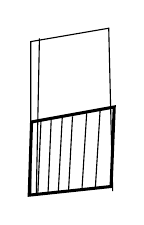
\begin{tikzpicture}[x=1cm,y=1cm]
\draw[thin] (0.02,0) -- (0.02,1.95) -- (1.01,2.12) -- (1.06,0.05);
\draw[thin] (0.09,0) -- (0.13,1.99);
\draw[line width=1.1pt] (0,0) -- (0.03,0.93) -- (1.08,1.12) -- (1.04,0.11) -- cycle;
\draw[thin] (0.11,0.03) -- (0.15,0.95);
\draw[thin] (0.24,0.04) -- (0.28,0.97);
\draw[thin] (0.37,0.05) -- (0.42,0.99);
\draw[thin] (0.50,0.06) -- (0.55,1.00);
\draw[thin] (0.67,0.07) -- (0.73,1.04);
\draw[thin] (0.84,0.09) -- (0.90,1.07);
\end{tikzpicture}}

\deleted{($(B,1)$ est bordant dans}

($\dot C$ est bordant dans \deleted{$B$} $(C\setminus\dot C)$)
Collier rigidifié

\uline{Conj} $\unsure{\Rightarrow|\to}$ Soit $B$ bordant dans $X$

a) $\exists$ Collier $(C,\dot C)$ donc aussi collier strict

b) ``L'espace'' des colliers stricts est contractile.

c) L'espace des \deleted{colliers \inserted{rigidifiés} et \unsure{stricts}}
\deleted{est fibré sur}
colliers \deleted{\unsure{stricts}} est contractile, ou en-
core : l'espace des autom. d'un
collier, induisant l'identité de $B$
(et ``libres'' sur $\dot C$) est contractile.

i.e. le choix d'un collier\inserted{strict}, ou d'un collier \inserted{strict} rigidifié,
ou d'une rigidification d'un collier, est
anodin.

\scanpage{149}
\mspage{2}
% archive foliation: 148
II) Soit $a\in X$. ``Cône'' autour de $a$ :
\[
a\in C\subset X,\qquad
\underbrace{\underset{\substack{\Vert\\Y}}{\dot C}\unsure{\subset}C}_{\substack{\text{sous-espaces}\\\text{modérés}}}
\qquad\text{tels que}
\]
\[
(C,\unsure{a})\xleftarrow[\sim]{\varphi}
\deleted{\unsure{C_\varphi}}\ \operatorname{Cone}(\deleted{Y}\inserted{\dot C})
\qquad(\text{avec }\varphi(\unsure{a|o})=\unsure{o|a}).
\]
Cône strict : $\dot C$ est bordant dans $X\setminus(C\setminus\dot C)$.

Cône rigidifié.

\uline{Conj} a) \unsure{Existe} cône

b) L'espace des cônes \inserted{stricts} est contractile

c) L'espace des rigidifications des
cônes est contractile i.e. l'espace
des autom. de $\operatorname{Con}(Y)$, qui sont
l'identité sur $Y$ et fixent $a$,
est contractile (\unsure{Alexandroff} ?)

Donc le choix d'un cône strict autour
de $a$, ou d'un cône strict rigidifié,
ou d'une \deleted{cône} rigidification sur un
cône donné, est anodin.

$\overline{\underline{\mathrm{III}}}$

Catégorie \inserted{$PB$} des paires $(X,B)$\quad $B$ bordant dans $X$

Catégorie \inserted{$PBCR$} des \deleted{paires} triples
$(X,B,C,\deleted{\unsure{\dot C}}\varphi)$, des
paires bordantes avec collier \inserted{strict} rigidifié

Catégorie $PBC$\quad $(X,B,C,\dot C)$\quad (paires bord. avec coll.)

Catégorie \inserted{$EP$} des paires $(X,a)$\quad $X$ pointé

\scanpage{150}
\mspage{3}
% archive foliation: 149
Catégorie \inserted{$EPCR$} des triples $(X,a,(C,\unsure{\psi|\varphi}))$
$(C,\unsure{\psi|\varphi})$ cône strict rigidifié

Catégorie $EPC$ des triples $(X,a,(C,\dot C))$.
espaces mod. pointés, \deleted{rigidifiés} cône strict

On a une cascade d'équivalences de cat.
\deleted{$\unsure{PB}$} $\infty$-isotopiques

\diagram{\begin{tikzcd}[row sep=4.4em,column sep=7em]
& PB
 \arrow[dl,bend right=18,very thick,"{\substack{\text{recoller }B\times I\text{ par}\\B\times\{0\},\ \unsure{\text{nouvelle}}\\\text{partie bordante }B\times\{1\}}}"']
 \arrow[dr,<->,bend left=18,"{\text{recoller Cône}(B)}"]
 \arrow[dddl,"{\mathrm{id}_{PB}}"',""{name=ida,pos=.85}]
 \arrow[dddr,"{\substack{\text{contraction}\\\text{de }B\text{ en}\\\text{un point}}}",""{name=idb,pos=.85}]
& \\
PBCR \arrow[rr,dashed] \arrow[d,"{\text{oubli rig.}}"'] && EPCR \arrow[d,"{\substack{\text{oubli rigidification}\\\text{cône}}}"] \\
PBC \arrow[rr,dashed] \arrow[d,"{\text{oubli collier}}"',""{name=fa}] && EPC \arrow[d,"{\text{oubli cône}}",""{name=fb}] \\
PB \arrow[rr] && EP
\arrow[Rightarrow,from=fa,to=ida,"\alpha","\sim"']
\arrow[Rightarrow,from=fb,to=idb,"\beta","\sim"']
\end{tikzcd}}

\margin{\uline{NB} Pour définir $\alpha$ et $\beta$, \unsure{composer}
les foncteurs envisagés (i.e. \unsure{les sources}) avec $PBR$}

\margin{Système des \unsure{11|14} foncteurs qui sont des
équivalences $\infty$-isotopiques}

\deleted{\unsure{IV}} \uline{Variantes} \deleted{Paires}
Multipaires bordantes ($B=\coprod_{i\in I}B_i$)
espaces multipointés ($I\hookrightarrow X$)
($I$ un \unsure{ensemble} fini variable)

\margin{\deleted{\unsure{IV}}}

\diagram{\begin{tikzcd}[row sep=4em,column sep=2.7em]
&& PB
 \arrow[dll,very thick,"{\text{recoller collier}}"']
 \arrow[d,"{\text{recoller cône}}"']
 \arrow[ddd,shift left=1.1ex,"{\deleted{\unsure{\text{ident.}}}}" near start,"{\text{identité}}" description,""{name=ia,pos=.9}]
 \arrow[dddrr,"{\text{contr. des }B}",""{name=ib,pos=.85}]
&& \\
PBCR \arrow[rr,very thick] \arrow[dr] && EPCR \arrow[dr,very thick] && \\
& PBC \arrow[rr,very thick] \arrow[dr,very thick,""{name=ga}] && EPC \arrow[dr,very thick,""{name=gb}] & \\
&& PB \arrow[rr] && EP
\arrow[Rightarrow,from=ga,to=ia,"{\deleted{\unsure{\alpha}}\ \unsure{\alpha}}","\sim"']
\arrow[Rightarrow,from=gb,to=ib,"\beta","\sim"']
\end{tikzcd}}

\uline{Scholie} : du pt de vue $\infty$-isotop.,
\deleted{il y a} \inserted{c'est}
pareil que de travailler avec l'une des
six catégories équivalentes.

\scanpage{151}
\mspage{4}
% archive foliation: 150
$\overline{\underline{\mathrm{IV}}}$
\uline{Voisinages tubulaires d'une partie}
modérée $Y$ d'un espace modéré $X$.

C'est par définition un cône strict
autour de $o$ de $X/Y$.

Construction : Soit $f:X\unsure{-|\longrightarrow}\mathbb R^+$
(fonction modérée) telle que
\[
f^{-1}(\{0\})=Y.
\]
On prend $V=f^{-1}([0,\varepsilon])$
$\varepsilon$ petit [et admissible], et
\[
\dot V=f^{-1}(\{\varepsilon\}).
\]

\margin{Choix du vois. tubulaire,
ou du vois. tub. rigidifié, est \uline{anodin}.
\unsure{Noter} que $\dot V$ bien défini en cat.
$\infty$-\unsure{isotopiques}\ldots}

Rigidification du voisinage tubulaire
($=$ du cône). Rigidification
$Y$-admissible : s'insère dans diagramme \inserted{(\unsure{comm})}

\diagram{\begin{tikzcd}[column sep=small,row sep=2em]
V & V-Y=V^*\simeq\dot V\times[0,1[
 \arrow[dl,leftrightarrow] \arrow[dr] & \\
X\simeq \arrow[dr] &
\bigl((X\setminus(\unsure{\dot V|V}\setminus\dot V))\amalg(\dot V\times I\deleted{\unsure{\varepsilon}})\bigr)
& \deleted{\unsure{\amalg}}\underset{\dot V\times\{1\}}{\unsure{\vee|\amalg}}\deleted{\unsure{\amalg}}Y, \\
& Y \arrow[ur,leftrightarrow] &
\end{tikzcd}}

par $\varphi:\dot V\times\{1\}\longrightarrow Y$ appl. modérée
(déterminée de façon unique par la
rigidification).

a) Rigidification $Y$-admissible existe

b) La classe d'homotopie de $\dot V\longrightarrow Y$
bien déterminée

Mais on voudrait plus précis.

\scanpage{152}
\mspage{5}
% archive foliation: 151

1°) Cas où $X$ équi-singulier autour de $Y$.
Je présume qu'on doit pouvoir prendre
$\varphi$ fibrant (``rigidification fibrante''),
et qu'on a une équivalence de catégories
$\infty$-isotopiques

\diagram{\begin{tikzcd}[column sep=small,row sep=large]
& \text{Syst. }(X',B,\deleted{\varphi}\inserted{Y},\varphi)
  \arrow[d,"\approx"]
& \begin{gathered}(X',B)\text{ paire bordante}\\
\varphi:B\longrightarrow Y\text{ morphisme}\\\text{fibrant}\end{gathered}\\
\begin{gathered}(X',B,Y,\varphi)\\
\longmapsto((X'\amalg_B Y,\varphi),Y)\end{gathered}
& (X,Y):\text{ paires équi-singulières.} &
\end{tikzcd}}

\uline{NB} les $X\setminus Y,Y$
\deleted{\unsure{non singuliers, alors}}
\inserted{réguliers}
doivent correspondre au cas où
$X'$ variété à bord $B$, et $Y$ régulier.

\margin{Je présume que $X\setminus Y$ régulier
implique que $Y$ régulier
(\unsure{au moins si} $Y\subset\overline{X\setminus Y}$)}

2°) Cas général (pas néc. équi-sing.).
Il faudrait arriver à imposer des
conditions suppl. sur $\varphi:\dot V\longrightarrow Y$,
pour assurer l'unicité \unsure{esselle}.
Peut être qque chose du genre
suivant : Pour $\unsure{\forall|\text{tout}}\ y\in Y$, si $c(y)=\operatorname{codim}_y(Y,X)$
alors $\dim\varphi^{-1}(y)=c(y)-1$
(\unsure{cas de figure} plus précis, local sur $\dot V$ \unsure{ald} de l'être sur $Y$

\scanpage{153}
\mspage{6}
% archive foliation: 152

On peut \unsure{rien|bien} trouver encore une
description de la catégorie $\infty$-isotopique
des paires \inserted{\unsure{quelconques}} $(X,Y)$, en termes
d'une catégorie $(X',B,\varphi:B\longrightarrow Y)$, où
$\varphi$ serait soumis à certaines conditions
(\unsure{reflétant} \inserted{p.ex.} l'exigence dimensionnelle
précédente).

\figure{
\begin{tikzpicture}[x=1cm,y=1cm]
\draw (0,0.45) -- (3.9,0.48);
\draw (1.15,-0.12) .. controls (0.80,0.23) and (1.75,0.68) .. (1.97,-0.03)
 -- (1.97,-0.27) -- (2.08,0.73)
 .. controls (2.39,0.27) and (2.74,0.33) .. (2.71,0.40)
 .. controls (2.68,0.51) and (1.54,0.36) .. (1.23,0.39);
\end{tikzpicture}}

Filtrations équidimensionnelles et
régulières d'un espace modéré.

Il y en a je présume une qui
est canonique, c'est la \deleted{\unsure{plus}}\inserted{\unsure{moins}} fine
de toutes. [\inserted{\unsure{Plus gén.}} Pour \deleted{\unsure{toute}} filtration
déjà donnée, il y a une filtration
\deleted{plus fine} canonique, régulière
équidimensionnelle, compatible
avec celle-ci] Les invariants de
dévissage de cette filtration sont \unsure{donc}
des invariants de la structure
modérée envisagée.

\scanpage{155}
% archive foliation: 154

Digressions combinatoires (pour Réflexions \unsure{H.4|A.4})

\uline{Chap 1} Géométrie des ens de cardinal $\leq4$

\margin{\uline{NB} Faire \unsure{polygônes} des sommets, et des côtés
\unsure{rigoureusement}...}

\uline{Chap 2} L'icosaèdre gauche : ses trois
\deleted{\unsure{géométriques}}\inserted{perspectives}

\deleted{Orientations \unsure{de} $\unsure{\omega(S)}$}
$\alpha(\unsure{F|E})\in\omega(S)$ défini par les trois perspectives.

\uline{Chap 3} Biicosaèdres : les trois perspectives.
\margin{\deleted{$\unsure{\mathrm{Bic}(S)}$}
\[
\mathrm{Ic}(S)\simeq
\underset{\substack{\Vert\\\mathrm{Bic}(S)}}{S^*}\times\omega(S)
\]}

\uline{Chap 4} Dualité des hexagrammes

\margin{par \uline{bihexagones}}

1. L'autodualité $\mathrm{Ens}_6\simeq\mathrm{Ens}_6$
\inserted{décrits} via
$\operatorname{Aut}(S)\xrightarrow{\sim}\operatorname{Aut}(S^*)$

Application aux groupes d'autom. des
biicosaèdres \deleted{resp.}\inserted{et} icos.

2. Structure biicosaédrale par coloriage des arêtes

3. L'autodualité (trois \uline{perspectives})
\[
\left.\begin{array}{ll}
\text{a)}&\forall s\in S,\quad s'\in S^*\qquad
 S\setminus\{s\}\simeq S^*-\{s'\}\\
\text{b)}&R\unsure{\subset|\in}\deleted{\unsure{\mathcal P_2}}
 \operatorname{Ar}(S)\times\operatorname{Ar}(S^*)\\
\text{c)}&\mathcal P_{3,3}(S)\simeq\mathcal P_{3,3}(S^*)
\end{array}\right\}\ \text{avec axiomes}
\]

4\deleted{\unsure{3}}. Le dictionnaire de la dualité
\[
\begin{array}{lll}
\text{A)}&\mathrm{Ens}_5\deleted{\unsure{\mathrm{Ens}}}
 \inserted{\simeq\mathrm{Ens}(1,5)}&\approxeq\mathrm{Biicos.}\\
&\mathrm{Ens}_5^+\simeq\mathrm{Ens}^+(1,5)&\approxeq\mathrm{Icos}\\[1ex]
\text{B)}&\mathrm{Ens}_2\times\mathrm{Ens}_4
 &\approxeq\mathrm{Ens}_{2,2,2}\approxeq\mathrm{Cub}_3\\[1ex]
\text{C)}&\underbrace{\mathrm{Ens}_{3,3}}_{\text{\unsure{ditrièdres|ditriades}}}
 &\approxeq\mathrm{Ens}_{3,3}\quad\text{dualité}
\end{array}
\]

\margin{\deleted{$\begin{gathered}
\text{A')}\ \mathrm{Bipent}\approxeq\mathrm{Biicos.}+\text{sommet}\\
\mathrm{Pent}\approxeq\mathrm{Icos.}+\unsure{\text{sommet}}\\
\text{B')}
\end{gathered}$}}

\margin{Notion \unsure{biditrièdres|biditriades} $\equiv$}

% The long left relocation arrow rises toward item 3.
\diagram{\begin{tikzcd}[column sep=small,row sep=large]
{} & {} & {}\\
\left[\begin{gathered}
\text{A')}\quad\mathrm{Biicos.}+\text{sommet}
\approxeq\deleted{\unsure{\mathrm{Ens}_{1,5}}\simeq\mathrm{Ens}_5}
\inserted{\unsure{\mathrm{Bipent}_5}}\\
\mathrm{Icos}+\text{---}\ \overset{\approx}{\longrightarrow}
\deleted{\mathrm{Ens}_{1,5}^{+}\simeq\mathrm{Ens}_5^{+}}
\mathrm{Pent}_5\\[2ex]
\text{B')}\quad\mathrm{Biicos}+\text{ar.}\approxeq
\deleted{\unsure{\mathrm{Ens}_2}}\times\mathrm{Car}\\[3ex]
\text{C')}\quad\mathrm{Biicos}+\text{biface}\simeq
\mathrm{Ens}_2\times\mathrm{Ens}_3
\end{gathered}\right.
\arrow[u,bend left=75]
& \deleted{\begin{gathered}
\overset{\approx}{\longrightarrow}\unsure{\mathrm{Ens}_2}\times\mathrm{Car}\\
\text{autodualité}\\
\text{de }\mathrm{Ens}_2\times\mathrm{Car}\\
\text{explicite}
\end{gathered}}
\arrow[loop above,leftrightarrow,looseness=3]
\arrow[dr]
&{}\\
\text{remonter à Chap 3} & \sim(\unsure{\text{Hexagones}})&
\text{
\begin{tikzpicture}[baseline=-.5ex]\draw (0,0) ellipse (.7cm and .23cm);\node at (0,0) {TSVP};\end{tikzpicture}}
\end{tikzcd}}

\margin{\diagram{\begin{tikzcd}[row sep=small,column sep=small]
&\approxeq\\
\text{compos}\arrow[ur]&\mathrm{Car}\arrow[u,"\deleted{\unsure{2}}"']
\end{tikzcd}}}

\diagram{\begin{tikzcd}
\alpha\times f &(\alpha,f)\arrow[l]
\end{tikzcd}}

\deleted{\unsure{5)}}

\scanpage{156}
% archive foliation: 155

\deleted{\unsure{5}}\inserted{$B_1$})
$\deleted{\unsure{S}}\ \mathrm{Car}(S)\simeq\mathrm{Car}(S^*)$

\figure{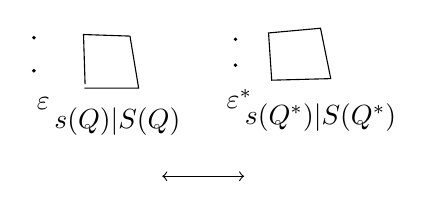
\begin{tikzpicture}[x=1cm,y=1cm]
\draw (0.65,0.55) -- (0.63,1.18) -- (1.22,1.16) -- (1.33,0.50) -- (0.64,0.50);
\fill (0,1.14) circle (0.025);\fill (0,0.72) circle (0.025);
\node at (0.12,0.30) {$\varepsilon$};
\node at (1.06,0.08) {$\unsure{s(Q)|S(Q)}$};
\draw (3.02,0.60) -- (2.98,1.20) -- (3.64,1.26) -- (3.77,0.62) -- cycle;
\fill (2.56,1.12) circle (0.025);\fill (2.56,0.79) circle (0.025);
\node at (2.61,0.36) {$\varepsilon^*$};
\node at (3.64,0.12) {$\unsure{s(Q^*)|S(Q^*)}$};
\draw[<->] (1.63,-0.62) -- (2.67,-0.62);
\end{tikzpicture}}

\margin{expliciter utilisant
\[
\left\{\begin{array}{l}
\varepsilon\wedge\varepsilon^*\wedge\omega(Q)=1\\
\omega(Q)\simeq\omega(Q^*)\\
Q^*\simeq\varepsilon\wedge Q\ ;\quad Q\simeq\varepsilon^*\wedge Q^*
\end{array}\right.
\]}

$C_1$) Relation avec la donnée d'un
\deleted{espace} plan affine $\unsure{V}$ sur $\mathbb F_3$
et de \deleted{$\unsure{\operatorname{card}P(V)}=4$},
$\operatorname{Card}(\unsure{E}=P(V))=4$, \deleted{Aut}
\[
\unsure{\mathfrak G|\mathfrak S}_{P(V)}\simeq
\underline{\operatorname{Aut}}(V)(\mathbb F_3)\simeq
\mathrm{GP}(\unsure{1|2},\mathbb F_3)
\]
et une partition \inserted{$(2,2)$ de $E$ (en \unsure{antipodismes})}

i.e. \unsure{Structure carrée} sur $E$.
\[
\operatorname{card}(E_i)=3\qquad i\in E
\]
\diagram{\begin{tikzcd}
E_i\times E_j & V\arrow[l,"\sim"'] &
\text{pour }i,j\in E\quad i\neq j
\end{tikzcd}}

\margin{\diagram{\begin{tikzcd}V\arrow[r,"p_i"']&E_i\end{tikzcd}}
$V\subset\prod E_i$}

\figure{\begin{tikzpicture}[x=1cm,y=1cm]
\fill (0.10,1.70) circle(0.025);\fill(0.25,2.03) circle(0.025);\fill(0.48,2.37) circle(0.025);
\fill (1.35,2.50) circle(0.025);\fill(1.77,2.44) circle(0.025);\fill(2.23,2.27) circle(0.025);
\fill (2.80,1.57) circle(0.025);\fill(2.71,1.17) circle(0.025);\fill(2.66,0.86) circle(0.025);
\fill (0.62,0.51) circle(0.025);\fill(1.04,0.36) circle(0.025);\fill(1.46,0.31) circle(0.025);
\fill(5.34,1.06) circle(0.025);\fill(5.56,1.07) circle(0.025);\fill(5.79,1.08) circle(0.025);\fill(6.00,1.09) circle(0.025);
\draw(5.22,1.01)..controls(5.30,0.91)and(5.40,0.97)..(6.26,1.00);
\end{tikzpicture}}

Groupe d'automorphismes \unsure{trilitaire}
d'ordre $3^3\times2^4=3.144$ \unsure{,}

Opère sur $\unsure{\mathfrak G|\mathfrak S}_{\varepsilon}$
\margin{$\varepsilon=\coprod_{i\in E}E_i$}

et laisse invariant \deleted{trois} un syst.
de $3$ sous-groupes $G_\alpha$
($\alpha\in\deleted{\unsure{\mathcal E}}\mathrm{Car}(E)=\mathrm{Antip.}(E)$)
Le stabilisateur d'un $G_\alpha$ est le groupe des
automorphismes d'une bi-ditriade. Opère
fidèlement sur $G_\alpha$, sous groupe d'ordre $\unsure{10|16}$ de
$\operatorname{Aut}(G_\alpha)$
\inserted{(d'ordre $\unsure{2.(8!)|2.(6!)}$)}

\margin{les $G_\alpha$ ont un
$3$-sous-groupe de Sylow \inserted{$V_0$} en commun, et
\deleted{\unsure{qui est}} \unsure{d'indice} \illegible{2}
\deleted{la \unsure{décomposition} \illegible{2} de $V$}
\deleted{et $\unsure{V/V_0|G/V_0}$ est le groupe du
\unsure{carré} \illegible{2}}
$N_{\unsure{\operatorname{Aut}G_\alpha}}(V_0)/V_0$
\unsure{opère} \illegible{2}
(groupe du carré)}

\scanpage{157}
% archive foliation: 156

\textcircled{$3'$}\quad $1,2,3$
\figure{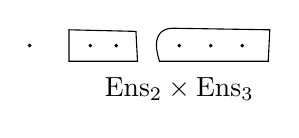
\begin{tikzpicture}[x=1cm,y=1cm]
\fill(0,0.2)circle(0.025);
\draw(0.5,0)--(0.5,0.4)--(1.35,0.38)--(1.37,0)--cycle;
\fill(0.77,0.2)circle(0.025);\fill(1.1,0.2)circle(0.025);
\draw(1.65,0)..controls(1.55,0.3)and(1.65,0.42)..(1.82,0.42)--(3.05,0.4)--(3.03,0)--cycle;
\fill(1.9,0.2)circle(0.025);\fill(2.3,0.2)circle(0.025);\fill(2.7,0.2)circle(0.025);
\node at(1.9,-0.35){$\mathrm{Ens}_2\times\mathrm{Ens}_3$};
\end{tikzpicture}}
\deleted{\unsure{biicosaèdres}}

\diagram{\begin{tikzcd}[column sep=small,row sep=small]
\textcircled{1}&(1,5)\arrow[r,leftrightarrow] &\text{(biicosaèdre)}&\\
\textcircled{2}& |[draw,ellipse]| 2,4\arrow[d,leftrightarrow,bend left=45]&
\unsure{\mathfrak G|\mathfrak S}_4\times\unsure{\mathfrak G|\mathfrak S}_2&\\
& |[draw,ellipse]| 2,2,2&
\begin{gathered}\text{i.e. cube (pas }\deleted{\unsure{\text{néc.}}}\text{ orienté)}\\
\text{ext. de }\unsure{\mathfrak G|\mathfrak S}_3\text{ par }\unsure{\mathfrak G|\mathfrak S}_2^3
\end{gathered}\arrow[r]&
\begin{gathered}\unsure{\text{en crée}}\ 2\text{ structures}\\
\text{biicos. i.e. }4\text{ str.}\\
\text{icos. formant deux}\\\text{paires d'}\unsure{\text{opposées}}\end{gathered}\\
\textcircled{3}& |[draw,ellipse]| 3,3\arrow[loop right,leftrightarrow]&
\text{ext. de }\unsure{\mathfrak G|\mathfrak S}_2\text{ par }\unsure{\mathfrak G|\mathfrak S}_3\times\unsure{\mathfrak G|\mathfrak S}_3&
\mathbb F_3^2\simeq\mathrm{Syl}_3
\arrow[phantom,from=2-1,to=3-1,"{\Bigg\{}" description]
\arrow[phantom,from=2-3,to=3-3,"{\Bigg\}}" description]
\end{tikzcd}}

\margin{\figure{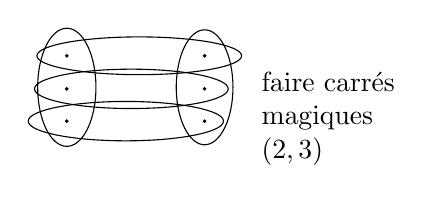
\begin{tikzpicture}[x=1cm,y=1cm]
\draw(1.3,1.05)ellipse(1.3 and .24);\draw(1.2,.63)ellipse(1.23 and .25);\draw(1.13,.22)ellipse(1.24 and .25);
\draw(.38,.65)ellipse(.37 and .75);\draw(2.13,.65)ellipse(.36 and .73);
\foreach \x in {.38,2.13}{\foreach \y in {.22,.63,1.05}{\fill(\x,\y)circle(.025);}}
\node[align=left]at(3.7,.25){faire \unsure{carrés}\\\unsure{magiques}\\$(2,3)$};
\end{tikzpicture}}}

\textcircled{$2'$}
\figure{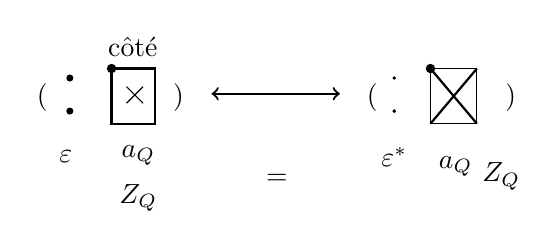
\begin{tikzpicture}[x=1cm,y=1cm]
\node at(-.35,.65){$($};\node at(1.38,.65){$)$};
\fill(0,.9)circle(.045);\fill(0,.48)circle(.045);
\node at(-.05,-.10){$\varepsilon$};
\draw[thick](.53,.32)rectangle(1.08,1.02);
\fill(.53,1.02)circle(.06);\draw(.72,.58)--(.93,.79);\draw(.72,.79)--(.93,.58);
\node at(.8,1.3){\unsure{côté}};\node at(.87,-.08){$a_Q$};\node at(.87,-.62){$Z_Q$};
\draw[<->,thick](1.80,.70)--(3.43,.70);
\node at(2.63,-.39){$=$};
\node at(3.84,.65){$($};\node at(5.60,.65){$)$};
\fill(4.12,.9)circle(.025);\fill(4.12,.48)circle(.025);
\node at(4.12,-.1){$\varepsilon^*$};
\draw(4.58,.32)rectangle(5.17,1.02);
\draw[thick](4.58,.32)--(5.17,1.02);\draw[thick](4.58,1.02)--(5.17,.32);
\fill(4.58,1.02)circle(.06);
\node at(4.9,-.22){$a_Q$};\node at(5.48,-.35){$Z_Q$};
\end{tikzpicture}}

\margin{$D_4\times\mathbb F_2\simeq\mathrm{Syl}_2$}
\[
\boxed{\begin{gathered}Q^*=\varepsilon\wedge Q^\vee\\
\deleted{\unsure{Q\simeq\varepsilon\wedge Q^*}}\end{gathered}}
\qquad\begin{gathered}\omega(Q)\simeq\omega(Q^*)=\omega\\
\deleted{\unsure{\varepsilon\wedge\varepsilon^*\wedge\omega\simeq1}}
\boxed{\varepsilon^*\wedge\varepsilon\wedge\omega\simeq1}
\end{gathered}
\]
\margin{\[
\overbrace{\varepsilon\wedge\operatorname{codiag}Q}^{\unsure{\omega(S)_6|\omega(S)}}
\simeq\overbrace{\varepsilon^*\wedge\operatorname{codiag}Q^*}^{\unsure{\omega(S^*)_6|\omega(S^*)}}
\]
i.e. $\underbrace{\varepsilon\wedge\varepsilon^*}_{\omega}\wedge
\operatorname{codiag}Q\wedge\operatorname{codiag}Q^*\simeq1$
d'où $\operatorname{codiag}Q^*\simeq\operatorname{diag}Q$}

\textcircled{$1''$}
\diagram{\begin{tikzcd}[column sep=large]
1+\text{bipentagone}\arrow[r,leftrightarrow]&1+\text{bipentagone}&\text{biicos. + sommet}\\
&\text{le }\simeq\ !&\\
1+\text{pentagone}\arrow[r,leftrightarrow]&1+\text{pentagone}&\text{icos. + sommet}
\end{tikzcd}}

\textcircled{$2''$}
\figure{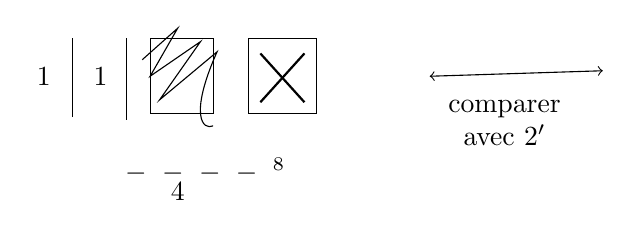
\begin{tikzpicture}[x=1cm,y=1cm]
\node at(0,.55){$1$};\draw(.36,.03)--(.36,1.03);\node at(.72,.55){$1$};\draw(1.05,0)--(1.05,1.03);
\draw(1.35,.08)rectangle(2.15,1.03);
\draw(1.25,.76)--(1.7,1.16)--(1.35,.55)--(1.99,.99)--(1.47,.25)--(2.2,.86)..controls(1.84,.05)and(2.02,-.14)..(2.15,-.08);
\draw(2.60,.08)rectangle(3.46,1.03);\draw[thick](2.75,.22)--(3.31,.84);\draw[thick](2.75,.84)--(3.31,.22);
\draw[<->](4.90,.55)--(7.10,.62);
\node[align=center]at(5.85,-.04){comparer\\avec $2'$};
\node at(2.05,-.65){$-\ -\ -\ -\ {}^8$};\node at(1.7,-.92){$\deleted{4}$};
\end{tikzpicture}}

\margin{biicos. + arête $\Vert$
\figure{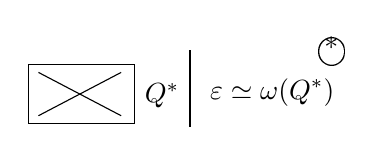
\begin{tikzpicture}[x=1cm,y=1cm]
\draw(0,0)rectangle(1.35,.75);\draw(.13,.1)--(1.18,.65);\draw(.13,.65)--(1.18,.1);
\node at(1.70,.36){$Q^*$};\draw[thick](2.05,-.04)--(2.05,.94);
\node at(3.1,.4){$\varepsilon\simeq\omega(Q^*)$};\node at(3.85,.92){$\textcircled{*}$};
\end{tikzpicture}}
icos. + arête \deleted{$\unsure{\varepsilon}$}
\figure{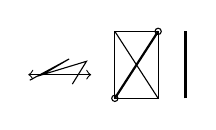
\begin{tikzpicture}[x=1cm,y=1cm]
\draw[<->](0,.3)--(.8,.3);\draw(.02,.23)--(.52,.5)--(.18,.3)--(.74,.47)--(.56,.18);
\draw(1.1,0)rectangle(1.65,.85);\draw[thick](1.1,0)--(1.65,.85);\draw(1.1,.85)--(1.65,0);
\draw(1.1,0)circle(.04);\draw(1.65,.85)circle(.04);\draw[very thick](2,0)--(2,.85);
\end{tikzpicture}}}

\textcircled{$3''$}
\figure{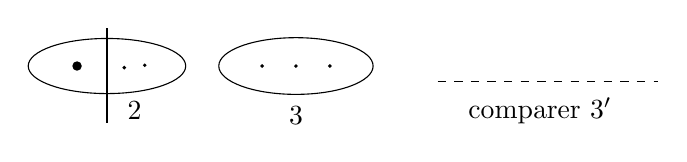
\begin{tikzpicture}[x=1cm,y=1cm]
\draw(1,.60)ellipse(1 and .35);\fill(.62,.6)circle(.06);\fill(1.22,.58)circle(.025);\fill(1.48,.61)circle(.025);
\draw(1,-.12)--(1,1.08);\node at(1.35,.04){$2$};
\draw(3.4,.60)ellipse(.98 and .36);\foreach\x in{2.97,3.4,3.83}{\fill(\x,.6)circle(.025);}\node at(3.4,-.03){$3$};
\draw[dashed](5.2,.4)--(8,.4);\node at(6.5,.03){comparer $3'$};
\end{tikzpicture}}
\deleted{$\unsure{a\ a'\ a\ v',\ b\ u'}$}

\margin{biicos. + biface \unsure{un prisme}
\figure{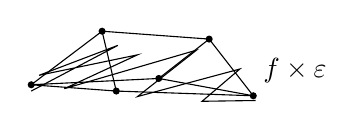
\begin{tikzpicture}[x=1cm,y=1cm]
\coordinate(A)at(0,0);\coordinate(B)at(.9,.68);\coordinate(C)at(1.08,-.08);
\coordinate(D)at(1.62,.08);\coordinate(E)at(2.26,.58);\coordinate(F)at(2.82,-.14);
\draw(A)--(B)--(C)--cycle;\draw(D)--(E)--(F)--cycle;\draw(A)--(D);\draw(B)--(E);\draw(C)--(F);
\foreach\p in{A,B,C,D,E,F}{\fill(\p)circle(.045);}
\draw(0,-.08)--(1.1,.5)--(.1,.12)--(1.35,.38)--(.42,-.05)--(2.1,.44)--(1.35,-.15)--(2.65,.2)--(2.17,-.21)--(2.85,-.2);
\node at(3.35,.18){$f\times\varepsilon$};
\end{tikzpicture}}
icos + face\quad \unsure{un prisme}\quad $f\times\{0,1\}$}

\figure{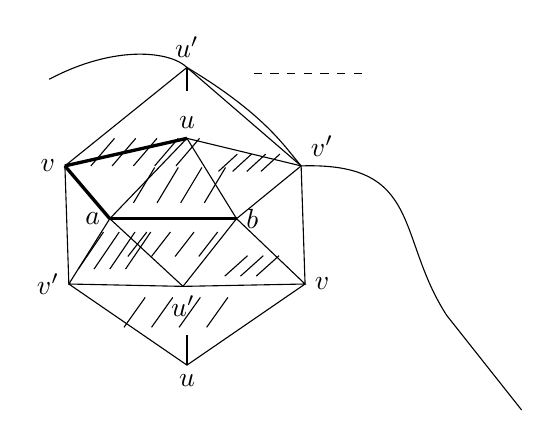
\begin{tikzpicture}[x=1cm,y=1cm]
\coordinate(T)at(2,3.8);\coordinate(U)at(2,2.9);\coordinate(L)at(.45,2.55);\coordinate(R)at(3.45,2.55);
\coordinate(A)at(1.02,1.88);\coordinate(B)at(2.63,1.88);\coordinate(LL)at(.50,1.05);\coordinate(RR)at(3.50,1.05);
\coordinate(UU)at(1.95,1.02);\coordinate(BT)at(2,.02);
\draw(T)--(L)--(LL)--(BT)--(RR)--(R)--cycle;
\draw(L)--(U)--(R);\draw(L)--(A)--(U)--(B)--(R);\draw(A)--(LL)--(UU)--(RR)--(B);\draw(A)--(UU)--(B);\draw(A)--(B);
\draw[very thick](L)--(U);\draw[very thick](L)--(A);\draw[very thick](A)--(B);
\foreach\x in{.78,1.05,1.32,1.59,1.86}{\draw(\x,2.55)--++(.30,.35);}
\foreach\x in{1.32,1.62,1.92,2.22}{\draw(\x,2.08)--++(.27,.45);}
\foreach\x in{2.40,2.58,2.76,2.94}{\draw(\x,2.48)--++(.24,.22);}
\foreach\x in{.62,.82,1.02,1.22}{\draw(\x,1.24)--++(.32,.47);}
\foreach\x in{1.25,1.55,1.85,2.15}{\draw(\x,1.40)--++(.24,.31);}
\foreach\x in{2.48,2.68,2.88}{\draw(\x,1.15)--++(.29,.26);}
\foreach\x in{1.20,1.55,1.90,2.25}{\draw(\x,.50)--++(.27,.38);}
\draw(T)--++(0,-.3);\draw(BT)--++(0,.38);
\node[above]at(T){$u'$};\node[above]at(U){$u$};\node[left]at(L){$\unsure{v}$};\node[above right]at(R){$v'$};
\node[left]at(A){$a$};\node[right]at(B){$b$};\node[left]at(LL){$v'$};\node[right]at(RR){$v$};\node[below]at(UU){$u'$};\node[below]at(BT){$u$};
\draw(.25,3.65)..controls(1.1,4.1)and(1.8,4.0)..(T)..controls(3,3.2)and(3.25,2.78)..(R)
..controls(5,2.60)and(4.65,1.65)..(5.30,.65)--(6.25,-.55);
\draw[dashed](2.85,3.72)--(4.25,3.72);
\end{tikzpicture}}

\unsure{Programme :} icosaèdre

\diagram{\begin{tikzcd}
\{a,b\}\wedge\{u,u'\}\arrow[r]&\{v,v'\}
\end{tikzcd}}
\deleted{$\unsure{\{a,b\}\wedge u}$}\qquad $a\wedge u=v$
\[
a\wedge v=u'
\]
\[
\{a,b\}\wedge
\underset{\operatorname{codiag}(Q)}{\underbrace{\{u,u'\}}\wedge\underbrace{\{v,v'\}}}
\simeq\deleted{\unsure{\omega(S)}}\operatorname{diag}Q
\]
\[
\{a\unsure{\wedge|,}b\}\simeq\omega(Q)
\]

\margin{\textcircled{*} choix d'une structure icosaédrale du
\unsure{G} biicosaèdre
$\simeq\operatorname{diag}(Q)$ / \unsure{Mais on}
$\simeq\unsure{\omega_\Delta|\omega}(S\amalg\varepsilon)
\simeq\omega(S)\wedge\varepsilon\simeq\operatorname{codiag}(Q)\wedge\varepsilon
\simeq\operatorname{diag}Q$ OK!}

\scanpage{158}
% archive foliation: 157

\deleted{$\unsure{IV''_5}$} $V''_4$ \deleted{Avenir-passé} \unsure{Durée}

\begin{center}
\begin{tabular}{rcl}
A v e n i r & - & p a s s é\\
destinée & - & histoire\\
pérennité & - & ancienneté\\
innovation & - & tradition (III)\\
\deleted{le nouveau} & \deleted{-} & \deleted{l'ancien}\\
\multicolumn{3}{l}{\deleted{\illegible{4}}}\\
\inserted{élan} & \inserted{-} & \inserted{enracinement (II)}
\end{tabular}
\end{center}

\deleted{$\unsure{IV''_6}$} $V''_5$ Espace-temps

\begin{center}
\begin{tabular}{rcl}
E s p a c e & - & t e m p s\\
étendue (ou distance) & - & durée\\
\deleted{ubiquité} & \deleted{-} & \deleted{éternité}
\end{tabular}
\end{center}

\margin{$\unsure{=\ ?\ ?}$}
\figure{\begin{tikzpicture}[x=1cm,y=1cm]
\draw (0,0)--(1.4,4.7);
\end{tikzpicture}}
\margin{\(\left\{\begin{array}{l}
\text{Complément t. d. m.}\quad\text{(+ harmonie)}\\
\text{mise en page liste}\\
\text{\unsure{fenêtre carrée}}\\
\text{dessins \ldots}
\end{array}\right.\)}

98 \quad (*) texte barré

\deleted{\unsure{99}} \quad (**) Plusieurs existences successives

100 \quad (*) texte barré

(**) Elle qui n'a point lu. Comparer note n° 162; \unsure{p. dep.} (\unsure{a}) p. \unsure{789}
``conviction et connaissance''

\figure{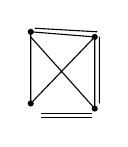
\begin{tikzpicture}[scale=.65]
\draw (0,0)--(0,1.4)--(1.25,1.3)--(1.25,-.1);
\draw (0,0)--(1.25,1.3) (0,1.3)--(1.25,-.1);
\draw (.2,-.2)--(1.2,-.2) (.2,-.28)--(1.2,-.28);
\draw (.08,1.47)--(1.3,1.4) (1.34,1.3)--(1.34,0);
\foreach \p in {(0,0),(0,1.4),(1.25,1.3),(1.25,-.1)}\fill \p circle(.06);
\end{tikzpicture}}

(***) \unsure{Ref. cours|Ref. aux} 1977. Frustration.

103 \quad (*) Autre \unsure{perspective}.

107 \quad (*) Mais pas \unsure{assez} pour la multiplication.

(**) \unsure{Copie d'élève}

(***) \unsure{cheminement} \illegible{1} \unsure{logique}.

110 \quad \unsure{Pensée} par \unsure{réciprocité}

\figure{\begin{tikzpicture}[x=.7cm,y=.7cm]
% Upper left pair of joined figures.
\coordinate (A) at (2,10);\coordinate (B) at (2.8,10.8);\coordinate (C) at (3.3,10);
\coordinate (D) at (1.3,7.8);\coordinate (E) at (3.2,8.1);\coordinate (F) at (2.3,8.8);
\draw[very thick] (A)--(B);\draw (A)--(C)--(B) (A)--(D)--(E)--(A) (D)--(F)--(A) (F)--(E);
\draw (1.25,7.7) .. controls (1.3,9) and (1.6,9.7) .. (A);
\foreach \p in {A,B,C}\fill (\p) circle(.05);
% Left-hand small fan and joined tetrahedral forms.
\draw (.5,8.7)--(-.6,8.1)--(.35,7.65);
\draw[very thick] (-.6,8.1) .. controls (-.1,8.05) and (.25,7.8) .. (.35,7.65);
\draw (.35,7.65)--(.05,6.4)--(1.05,6.15)--(1.45,6.95)--cycle;
\draw (.35,7.65)--(1.05,6.15) (.05,6.4)--(1.45,6.95) (.35,7.65)--(.8,6.85)--(.05,6.4) (.8,6.85)--(1.05,6.15);
\draw[very thick] (.35,7.65)--(.8,6.85);
% Middle-left diamond.
\coordinate (a) at (4,7.6);\coordinate (b) at (3,5.95);\coordinate (c) at (5.1,5.9);\coordinate (d) at (4.65,4.55);
\draw (a)--(b)--(d)--(c)--cycle (a)--(d) (b)--(c);
\draw (b) .. controls (4,6.2) and (4.6,6.1) .. (c);
\draw[very thick] (a)--(c) (c)--(d) (a)--(d);
\fill (b) circle(.06);\draw (c) circle(.1);
\node[above] at (a) {$a$};\node[left] at (b) {$b$};
% Heavily retraced central complex.
\coordinate (p) at (8.2,8.05);\coordinate (q) at (10.1,8.6);\coordinate (r) at (9.35,7.5);
\coordinate (s) at (8.7,6.35);\coordinate (t) at (10,6.25);\coordinate (u) at (9.6,5.2);
\draw[line width=2pt] (p)--(q)--(r)--cycle (p)--(s)--(t)--(r)--(s) (s)--(u)--(t);
\draw (p)--(t) (r)--(u) (s)--(q);
\foreach \x in {8.55,8.7,8.85,9,9.15}\draw (\x,7.8)--(\x+.25,7.45);
\foreach \x in {9.25,9.4,9.55,9.7}\draw (\x,7.15)--(\x-.05,6.35);
\foreach \x in {9,9.15,9.3,9.45,9.6,9.75}\draw (\x,6.25)--(9.6,5.3);
\draw (9.3,5.05)--(10.6,5.05) (9.3,4.98)--(10.6,4.98);
\node[above left] at (p) {$c'$};\node[above] at (q) {$\unsure{v}$};\node[left] at (r) {$a$};
\node[left] at (s) {$b$};\node[right] at (t) {$c$};\node[below] at (u) {$u$};
\node at (10.5,5.2) {$\deleted{\unsure{u}}$};
% Lists to the right of the complex.
\node[draw,ellipse,inner sep=2pt] at (12.15,9.4) {$abc$};
\node at (12.15,8.7) {$bcu$};
\node at (12.15,8) {$acu$};\draw (11.9,8) ellipse(.4 and .25);
\node at (12.15,7.3) {$abc'$};
\node at (13.1,6.6) {$\unsure{c'au}\quad\text{ou}\quad c'av$};
\node at (13.1,5.9) {$\unsure{c'bu}\quad\text{ou}\quad c'bv$};
\node[align=left] at (15,9.1) {$ac$\\$bc$\\$ab$\\$c'a$\\$c'b'$};
% Lower left figure and hatched quadrilateral.
\draw (.1,4.2)--(.3,2.9)--(1.8,2.8)--(1,1.9)--cycle;
\draw (.3,2.9)--(1.15,4.1)--(1.8,2.8) (1.15,4.1)--(1,1.9);
\draw (-.1,4.5)--(1,4.3) (-.1,4.5)--(.1,3.1);
\foreach \x in {.1,.25,.4,.55,.7}\draw (\x,4.35)--(\x+.12,3.35);
\foreach \x in {.65,.8,.95,1.1,1.25}\draw (\x,3.15)--(1.25,3.8);
\draw (.4,2.8)--(1,2.15) (.6,2.8)--(1.3,2.5);
% Long diamond at the bottom.
\coordinate (h) at (6.6,4.15);\coordinate (i) at (6.05,1.65);\coordinate (j) at (7.35,1.7);\coordinate (k) at (6.9,-.85);\coordinate (l) at (6.95,.3);
\draw (h)--(i)--(k)--(j)--cycle (i)--(j) (h)--(l) (i)--(l)--(j);
\draw (i) .. controls (6.25,.6) and (6.65,-.9) .. (k) (j) .. controls (7.5,.4) and (7.3,-.6) .. (k);
\foreach \x in {6.48,6.56,6.64,6.72}\draw (\x,3.1)--(\x+.24,3.5);
\node[left] at (i) {$a$};\node[right] at (j) {$b$};\node[above] at (k) {$\unsure{c}$};
% Lower middle-right bent figure.
\draw (10.2,4.05)--(10.9,3.65)--(11.65,2.3)--(11,1.25)--cycle (10.2,4.05)--(10.6,2.6)--(11.65,2.3) (10.6,2.6)--(11,1.25) (10.9,3.65)--(11,1.25);
\draw (9.95,3.2)--(9.95,4.2)--(10.2,4.05);
\foreach \x in {10.35,10.5,10.65,10.8,10.95}\draw (\x,3.6)--(\x-.1,2.7);
% Isolated triangular stroke and small right diamond.
\draw (14.1,4.15)--(14.65,3.2) (14.1,4.15)--(14.1,2.35)--(14.65,3.15);
\node at (13.8,2.85) {$*$};
\draw (16.8,4.9)--(16.15,4.1)--(16.6,3)--(17.15,4.05)--cycle (16.15,4.1)--(17.15,4.05) (16.8,4.9)--(16.6,3);
\foreach \x in {16.35,16.5,16.65}\draw (\x,4.15)--(16.8,4.8);
\draw (16.35,3.65)--(16.6,4) (16.5,3.4)--(16.8,4);
\end{tikzpicture}}

\scanpage{159}
% archive foliation: 158

\uline{Trialité des bi-di-triades}

On peut voir la structure \unsure{des deux parties}, soit par un \unsure{ens.}: 9 éléments $V$ (plan affine sur $\mathbb F_3$), soit par l'autre: 12 éléments $E$ (ens des droites de $V$). Relations d'incidence entre $E$ et $V$.

\margin{NB $E$ est \unsure{un} plan projectif sur $\mathbb F_3$, privé d'un \unsure{de ses} \unsure{points|point}.}

A) La structure sur $V$ revient à la donnée d'une partie $E$ de $\unsure{\mathcal P|\mathrm P}_3(V)$, telle que
\[
\left\{\begin{array}{l}
\operatorname{card}E=12\\
\forall a,b\in E,\ \text{on a}\quad \operatorname{card}a\cap b\leq1
\end{array}\right.
\]
\deleted{\unsure{(en fait}}

\deleted{\unsure{B)}}

B) Structure sur $E$: 1) partition en quatre classes de 3 éléments (\unsure{suivant} les quatre directions de droites)
\[
E=\coprod_{i\in I}E_i
\]

2) \deleted{Ens} $V$ de parties à 4 élts de $E$. (ens des droites passant par un point \inserted{de $V$}) avec les propriétés

a) Tout \deleted{\unsure{droite}} $D\in V$ rencontre chaque $E_i$ en \inserted{(au moins)} un \uline{pt} (\unsure{NB}: \inserted{au plus} un, \deleted{seul} \inserted{\unsure{revient au $=$)}} \deleted{(de $D$)}
\[
D\longrightarrow I\quad\text{est bijectif})
\]

b) Si $D,D'\in V$, $D\neq D'$, alors $\operatorname{card}D\cap D'=1$

\margin{\uline{NB} b) résulte de a) et c)}

c) Si $a,b\in E$ n'appartiennent pas à un même $E_i$, $\exists$ unique $D\in V$ qui y passe. (unicité provient d'ailleurs de b))

\margin{En introduisant $\widehat E\inserted{=E\coprod\{\infty\}}$ et
\[
\widehat V=V\coprod\left\{\begin{array}{l}
\text{ens des parties de }\widehat E\text{ de la forme}\\
E_i\cup\{\infty\}
\end{array}\right\}
\]
Ceci peut se dire: \deleted{\unsure{chaque}} deux ``droites'' distinctes $(\in\widehat V)$ se rencontrent en un point unique.}

\uline{NB} c implique déjà que $\operatorname{card}V=\unsure{9}$, et compte tenu de a), que par $\forall$ point $a\in E$ passent \unsure{exact$^t$} 3 ``droites''.

\scanpage{160}
% archive foliation: 159

Géométrie des ens. finis (de card $\leq\unsure{3}$) \hfill (Plan)

\uline{I} Ens: deux éléments

1. Produit contracté

\margin{(deux interprétations)
\[
\unsure{\mathfrak G|\mathfrak S}_2\simeq\pm1\simeq\mathbb Z/2\mathbb Z\simeq\mathbb F_3^*
\]}
\figure{\begin{tikzpicture}\draw[->] (2.2,.7) .. controls (.7,.8) and (.1,.6) .. (0,0);\end{tikzpicture}}

2. Orientation d'un ens fini $\{\omega(E)\}$. Associativité, lien avec orientation des vectoriels réels, ou des vectoriels orthogonaux \inserted{(car $\neq2$)}, ou des vectoriels sur $\mathbb F_3$.

3. Hypercubes et antipodismes. Orientation \unsure{dualité}

4. Carrés (sans lien avec carrés et cubes ordinaires)

\uline{II} Ens: trois éléments

1. 2-vectoriels sur $\mathbb F_2$ (ou \deleted{\unsure{espace}} \inserted{droite} projectif sur $\mathbb F_2$):
\[
\unsure{\mathfrak G|\mathfrak S}_3\simeq\mathrm{GL}(2,\mathbb F_2)\simeq\mathrm{SL}(2,\mathbb F_2)\simeq\mathrm{GP}(1,\mathbb F_2)
\]

2. Droites affines sur $\mathbb F_3$. Application aux ditriades, biditriades.
\[
\unsure{\mathfrak G|\mathfrak S}_3\simeq\operatorname{Aff}(1,\mathbb F_3)\ (\longrightarrow\mathbb F_3^*\simeq\pm1)
\]

\deleted{3. Quadritriades (ou tri-biditriades)}

\diagram{\begin{tikzcd}[column sep=small]
1\arrow[r]&\unsure{\mathfrak G|\mathfrak S}_3\unsure{\times}\unsure{\mathfrak G|\mathfrak S}_3\arrow[r]&\begin{gathered}\text{Aut d'une}\\\text{bi-di-triade}\end{gathered}\arrow[r]&\unsure{\mathbb Z_2|\mathfrak G_2}\arrow[r]&1
\end{tikzcd}}
\figure{\begin{tikzpicture}\draw[->] (1.5,0).. controls (.4,0) and (.8,.7) ..(.2,1.7);\end{tikzpicture}}

\uline{III} Ens: quatre éléments

\figure{\begin{tikzpicture}[x=1cm,y=1cm]\draw (0,.65) .. controls (.55,.65) and (.25,0) .. (.85,0) -- (4.5,0) .. controls (5.15,0) and (5.45,-.1) .. (5.7,-.65);\end{tikzpicture}}

\uline{1}. \deleted{Espace} \inserted{Plan} affine sur $\mathbb F_2$:
\[
\unsure{\mathfrak G|\mathfrak S}_4\simeq\operatorname{Aff}(2,\mathbb F_2)
\]

2. Lien avec cubes:
\[
\mathrm{Ens}_4\times\mathrm{Ens}_2\approxeq\underline{\mathrm{Cub}}_3
\]
\[
\unsure{\mathfrak G|\mathfrak S}_4\simeq\operatorname{Aut}^+(\mathrm{Cub}_3)\simeq\deleted{\unsure{\mathrm{GO}_3(\mathbb F_3)}}\quad\begin{gathered}
\text{aut. d'un vect. de dim}\\
\text{3 sur }\mathbb F_3\text{ qui \unsure{invarie}}\\
\text{un \unsure{syst.} de trois}\\
\text{droites formant base}
\end{gathered}
\]

3. Lien avec rapports anharmoniques

4. Droites projectives sur $\mathbb F_3$\quad $\unsure{\mathfrak G|\mathfrak S}_4\simeq\mathrm{GP}(1,\mathbb F_3)$

5. Les quadritriades (ou bi-di-triades).

\diagram{\begin{tikzcd}[column sep=small]
1\arrow[r]&\bigl(\unsure{\mathfrak G|\mathfrak S}_3\times\unsure{\mathfrak G|\mathfrak S}_3\bigr)'\arrow[r]\arrow[d,equal]&\begin{gathered}\text{Aut d'une}\\\text{quadritriade}\end{gathered}\arrow[r]\arrow[d,"\simeq" description,draw=none]&\unsure{\mathfrak G|\mathfrak S}_4\arrow[r]&1\\
&\{(\unsure{\sigma},\unsure{\sigma'})\mid\epsilon(\unsure{\sigma})=\epsilon(\unsure{\sigma'})\}&\operatorname{Aff}(2,\mathbb F_3)&&
\end{tikzcd}}

$\overline{\underline{\mathrm{IV}}}$ Ens: 5 éléments

\inserted{Droite proj. sur un corps à 4 éléments}

1. $\unsure{\mathfrak G|\mathfrak S}_5^+\simeq\mathrm{GP}(1,\mathbb F_4)$

\margin{$\unsure{\mathfrak G|\mathfrak S}_5\simeq$ Aut. droite projective sur un corps à 4 éléments \uline{non} \uline{précisé}}

\deleted{\unsure{ens}} ($E$ droite proj. sur $k\simeq\mathbb F_4$ alors
\[
\omega(E)\simeq(k^*\setminus\{1\})=\text{ens des deux gén. de }k\text{ sur }\mathbb F_2
\]
Expliciter rapports anharmoniques

2. $\unsure{\mathfrak G|\mathfrak S}_5\simeq\mathrm{GP}(1,\mathbb F_5)$ sera développé avec \unsure{th$^{rie}$} biicosaèdre

\scanpage{161}
% archive foliation: 160

$\overline{\underline{\mathrm V}}$ Théorie combinatoire des ens: 6 éléments et des biicosaèdres [peut être \unsure{scindé} en deux: A) Icosaèdre et biicosaèdre

B) géométrie des ens: 6 éléments]

Voir plan détaillé ailleurs\ldots

\deleted{\unsure{VI}}

\uline{Appendice} Polygones combinatoires.

Pour bien faire, il faudrait un exposé sur les réalisations géométriques des configurations envisagées ici\ldots

\scanpage{276}
% archive foliation: 275

\begin{center}
Rapport de la Commission relative au

recrutement des enseignants
\end{center}

I. Organisation du Département de Mathématique.

Le \uline{Département de Mathématique} de la Faculté des Sciences d'Orsay se compose d'une \uline{Ecole de Mathématique} et d'un \uline{Laboratoire de Mathématique}

1°/ L'\uline{Ecole de Mathématique} a la responsabilité des enseignements de premier et second cycle, y compris les enseignements non classiques qu'elle a la charge de développer en collaboration avec les autres départements de la Faculté.

2°/ Le \uline{Laboratoire de Recherche Mathématique} a la responsabilité des enseignements de troisième cycle et, d'une façon générale, de toutes les activités ayant pour but de faire de l'ensemble du Département un milieu favorable à la production mathématique.

Tout enseignant du Département de Mathématique, à un moment déterminé, appartient à l'une ou l'autre des deux sections. Les qualifications professionnelles requises pour être membre permanent de l'une ou l'autre des deux sections sont différentes.

3°/ Les décisions concernant l'organisation de l'enseignement, les nominations à des postes d'enseignement ou de recherche, les éventuels changements organiques à apporter au département de Mathématique, sont prises par l'\uline{Assemblée du département de Math.} de la Fac. des Sc.

\scanpage{277}
\margin{\unsure{2}}
% archive foliation: 276

d'Orsay. Celle-ci est formée

a) des maîtres de conférences et professeurs des deux sections (Laboratoire de Math. et Ecole de Math.)

b) des assistants et maîtres assistants ou de leurs représentants élus, à raison d'un sixième au plus de l'Assemblée.

c) des représentants élus des étudiants, pour un tiers de l'Assemblée.

Les décisions sont prises à la majorité absolue des votes exprimés, sauf pour les nominations ou pour les changements organiques, pour lesquels une majorité des deux tiers des votes exprimés est requise.

4°/ a) \uline{Obligations} des membres du \uline{Laboratoire de Recherche}.

Les obligations d'enseignement de Maîtres de Conférences et Professeurs sont de trois heures hebdomadaires dont la moitié consiste obligatoirement en un cours de 3\textsuperscript{ème} cycle, l'autre moitié pouvant être

--- soit un autre cours de 3\textsuperscript{ème} cycle

--- soit la direction d'un séminaire

--- soit un enseignement dans le cadre de l'Institut d'Enseignement (de préférence dans la Maîtrise de Mathématiques)

En outre la recherche et la direction de recherches font partie des obligations des Maîtres de Conférences et Professeurs

b) \uline{Obligations} des membres de l'\uline{Ecole de Mathématique}.

Le service d'un Maître de Conférences ou Professeur de

\scanpage{278}
% archive foliation: 277

l'Ecole de Mathématique \unsure{est de} 6 heures hebdomadaires, est dans ses attributions d'être le conseiller pédagogique des jeunes assistants et maître-assistants.

5°/ Il appartient à chacun des Maîtres de Conférences et Professeurs mathématiciens de la Faculté des Sciences d'Orsay en fonctions avant la rentrée d'Octobre 1968 de décider de son affectation au Laboratoire de Recherche ou à l'Ecole de Mathématiques, à titre permanent. \uline{Il est entendu qu'en cas de déséquilibre provisoire de l'ensemble des deux sections au profit du Laboratoire de Recherche, la vocation spéciale des membres de celui-ci ne pourra être respectée que dans la mesure où elle n'entre pas en conflit avec les impératifs de l'enseignement à assurer.}

$\overline{\underline{\mathrm{II}}}$ Critères de nomination.

La qualification nécessaire pour être nommé Maître de Conférence dans l'une ou l'autre section du Département de Mathématiques est le titre de Docteur ès Sciences Mathématiques, mention ``Enseignement'' pour les candidats à l'Ecole de Mathématique, mention ``Recherche'' pour les candidats au Laboratoire de Recherche Mathématique.

$\overline{\underline{\mathrm{III}}}$ Recrutement.

1°/ La nomination à tout poste d'enseignant ou de chercheur dans l'une ou l'autre section du département de

\scanpage{279}
\margin{\unsure{4}}
% archive foliation: 278

Math. (Laboratoire, Ecole) est décidée par l'Assemblée du département de Math.

2°/ La nomination des assistants et Maître-Assistants et la promotion des assistants au poste de Maître-\unsure{Assistant} peut être décidée le cas échéant par une Commission désignée par l'Assemblée. Cette Commission est formée d'enseignants et de représentants d'étudiants du département de Math. Ces derniers comprendront au moins un tiers et au plus une moitié des membres de la Commission et, il est entendu que le plus grand compte sera tenu de l'avis exprimé par ces représentants. La nomination ou la promotion est décidée sur avis favorable d'au moins deux tiers des membres de la Commission.

3°/ La nomination des maîtres de conférences ou des professeurs se fait par l'Assemblée réunie en session plénière. Elle est décidée sur avis favorable de deux tiers au moins des membres votants.

4°/ Dans le cas d'une nomination de Maître de Conférences ou de professeur à l'Ecole de Mathématique, les représentants des étudiants ont un droit de Véto qui devient effectif \unsure{si} deux tiers au moins des représentants d'étudiants se prononcent pour le véto.

5°/ Dans le cas d'une nomination au Laboratoire de Mathématique, et si une majorité des membres de ce laboratoire le demande, la décision est confiée à une Commission désignée par l'Assemblée.

\scanpage{280}
% archive foliation: 279

\unsure{Cette} Commission comprend tous les maîtres de conférences et professeurs du Laboratoire de Mathématique qui formeront au moins deux tiers de ladite Commission. Celle ci pourra inclure également, le cas échéant, des chercheurs détachés du CNRS au laboratoire de Math. et des Maître de conférence et professeurs de l'Ecole de Mathématique ayant compétence pour juger le candidat. La nomination est faite sur avis favorable de deux tiers au moins des membres de la Commission.

IV Détachements et changements de Sections.

1°/ Les membres du personnel enseignant de l'Ecole de Mathématique ont droit, tous les 4 ans, à un détachement auprès du Laboratoire, pour une durée d'un semestre. Ils n'ont aucune obligation d'enseignement pendant cette période.

Sur leur demande, et avec l'accord de l'Assemblée du Département, ils peuvent être détachés auprès du laboratoire pour une période d'un an \unsure{renouvelable}. Cette possibilité sera offerte, en \unsure{particulier}, aux enseignants, Docteurs d'Enseignement ou \unsure{non}, désirant obtenir la qualification nécessaire pour faire partie du laboratoire à titre \unsure{permanent}.

2°/ Les membres du personnel enseignant du Laboratoire \unsure{peuvent}, sur leur demande, et avec l'accord de l'\unsure{Assemblée} du Département, être détachés auprès de l'Ecole pour une période d'un an renouvelable.

\scanpage{281}
\mspage{-6-}
% archive foliation: 280

Ils ont, durant cette période, les mêmes obligations que le personnel enseignant de l'Ecole de Mathématique.

3°/ Le passage définitif d'une section à l'autre du Département est régi par les mêmes modalités qu'une première nomination.

\begin{center}\texttt{+=+=+=+=+=+}\end{center}
